\documentclass[11pt,letter]{article}
%-------------------------
\usepackage{amsmath,amssymb}

\usepackage{amsthm}
\usepackage{mathrsfs}
\usepackage{bm}
\usepackage{ascmac} 
\usepackage{amsmath}
\usepackage{natbib} %
\usepackage{fancybox}
\usepackage{float}
\usepackage{booktabs} 
\usepackage{bm,xstring}
\usepackage{tabularx}
\usepackage{graphicx}
%\usepackage{mediabb}
\usepackage{lipsum}
\usepackage {pdfpages}
\usepackage{booktabs}
\usepackage{array}
\usepackage{paralist}
\usepackage{verbatim}
\usepackage{subfig} 
\usepackage{ascmac}
\usepackage{amsthm}
\usepackage{multirow}
\usepackage{amsmath}
\usepackage{natbib}
\usepackage{longtable}
\usepackage{hhline}
\usepackage{tabularx}
\usepackage{booktabs}
%\usepackage[T1]{fontenc}
\usepackage{textcomp}
\usepackage{here}
\usepackage{setspace}
\usepackage{color}
\usepackage{url}
\usepackage{xcolor}
%\usepackage{filecontents}
\usepackage{setspace}
\usepackage{fancyhdr}
\usepackage{titling}
\usepackage{titlesec}
\usepackage{sectsty}
\usepackage{listings}
\usepackage[many]{tcolorbox}
\usepackage[framemethod=TikZ]{mdframed}
\usepackage[dvipdfmx]{}
%\usepackage[dvipdfmx]{color}
\usepackage{epstopdf}
%\usepackage[dvipdfmx]{color}

\usepackage{bbm}
\usepackage{pdflscape}
\newcommand{\vect}[1]{\boldsymbol{\mathbf{#1}}}

%%%%%%%%%%%%%%%%%%%%%%%%%%%%%%
%Theorem
\newcounter{theo}[section] \setcounter{theo}{0}
\renewcommand{\thetheo}{\arabic{theo}}
\newenvironment{theo}[2][]{%
\refstepcounter{theo}%
\ifstrempty{#1}%
{\mdfsetup{%
frametitle={%
\tikz[baseline=(current bounding box.east),outer sep=0pt]
\node[anchor=east,rectangle,fill=gray!20]
{\strut Theorem~\thetheo};}}
}%
{\mdfsetup{%
frametitle={%
\tikz[baseline=(current bounding box.east),outer sep=0pt]
\node[anchor=east,rectangle,fill=gray!20]
{\strut Theorem~\thetheo:~#1};}}%
}%
\mdfsetup{innertopmargin=10pt,linecolor=gray!20,%
linewidth=2pt,topline=true,%
frametitleaboveskip=\dimexpr-\ht\strutbox\relax
}
\begin{mdframed}[]\relax%
\label{#2}}{\end{mdframed}}
%%%%%%%%%%%%%%%%%%%%%%%%%%%%%%
%Lemma
\newcounter{lem}[section] \setcounter{lem}{0}
\renewcommand{\thelem}{\arabic{section}.\arabic{lem}}
\newenvironment{lem}[2][]{%
\refstepcounter{lem}%
\ifstrempty{#1}%
{\mdfsetup{%
frametitle={%
\tikz[baseline=(current bounding box.east),outer sep=0pt]
\node[anchor=east,rectangle,fill=gray!50]
{\strut Lemma~\thelem};}}
}%
{\mdfsetup{%
frametitle={%
\tikz[baseline=(current bounding box.east),outer sep=0pt]
\node[anchor=east,rectangle,fill=gray!50]
{\strut Lemma~\thelem:~#1};}}%
}%
\mdfsetup{innertopmargin=10pt,linecolor=gray!50,%
linewidth=2pt,topline=true,%
frametitleaboveskip=\dimexpr-\ht\strutbox\relax
}
\begin{mdframed}[]\relax%
\label{#2}}{\end{mdframed}}
%%%%%%%%%%%%%%%%%%%%%%%%%%%%%%
%Assumption
\newcounter{asm}[section] \setcounter{asm}{0}
\renewcommand{\theasm}{\arabic{section}.\arabic{asm}}
\newenvironment{asm}[2][]{%
\refstepcounter{asm}%
\ifstrempty{#1}%
{\mdfsetup{%
frametitle={%
\tikz[baseline=(current bounding box.east),outer sep=0pt]
\node[anchor=east,rectangle,fill=gray!50]
{\strut Assumption~\theasm};}}
}%
{\mdfsetup{%
frametitle={%
\tikz[baseline=(current bounding box.east),outer sep=0pt]
\node[anchor=east,rectangle,fill=gray!50]
{\strut Assumption~\thelem:~#1};}}%
}%
\mdfsetup{innertopmargin=10pt,linecolor=gray!50,%
linewidth=2pt,topline=true,%
frametitleaboveskip=\dimexpr-\ht\strutbox\relax
}
\begin{mdframed}[]\relax%
\label{#2}}{\end{mdframed}}
%%%%%%%%%%%%%%%%%%%%%%%%%%%%%%
%Definition
\newcounter{defn}[section] \setcounter{defn}{0}
\renewcommand{\thedefn}{\arabic{section}.\arabic{defn}}
%\renewcommand{\thedefn}{\arabic{defn}}
\newenvironment{defn}[2][]{%
\refstepcounter{defn}%
\ifstrempty{#1}%
{\mdfsetup{%
frametitle={%
\tikz[baseline=(current bounding box.east),outer sep=0pt]
\node[anchor=east,rectangle,fill=gray!50]
{\strut Definition~\thedefn};}}
}%
{\mdfsetup{%
frametitle={%
\tikz[baseline=(current bounding box.east),outer sep=0pt]
\node[anchor=east,rectangle,fill=gray!50]
{\strut Definition~\thedefn:~#1};}}%
}%
\mdfsetup{innertopmargin=10pt,linecolor=gray!50,%
linewidth=2pt,topline=true,%
frametitleaboveskip=\dimexpr-\ht\strutbox\relax
}
\begin{mdframed}[]\relax%
\label{#2}}{\end{mdframed}}

%%%%%%%%%%%%%%%%%%%%%%%%%%%%%%
%Proof
\newcounter{prf}[section]\setcounter{prf}{0}
\renewcommand{\theprf}{\arabic{section}.\arabic{prf}}
\newenvironment{prf}[2][]{%
\refstepcounter{prf}%
\ifstrempty{#1}%
{\mdfsetup{%
frametitle={%
\tikz[baseline=(current bounding box.east),outer sep=0pt]
\node[anchor=east,rectangle,fill=gray!50]
{\strut Proof~\theprf};}}
}%
{\mdfsetup{%
frametitle={%
\tikz[baseline=(current bounding box.east),outer sep=0pt]
\node[anchor=east,rectangle,fill=gray!50]
{\strut Proof~\theprf:~#1};}}%
}%
\mdfsetup{innertopmargin=10pt,linecolor=gray!50,%
linewidth=2pt,topline=true,%
frametitleaboveskip=\dimexpr-\ht\strutbox\relax
}
\begin{mdframed}[]\relax%
\label{#2}}{\qed\end{mdframed}}
%%%%%%%%%%%%%%%%%%%%%%%%%%%%%%
%%%%%%%%%%%%%%%%%%%%%%%%%%%%%%
%Note
\newcounter{notes}[section] \setcounter{notes}{0}
\renewcommand{\thenotes}{\arabic{notes}}
\newenvironment{notes}[2][]{%
\refstepcounter{notes}%
\ifstrempty{#1}%
{\mdfsetup{%
frametitle={%
\tikz[baseline=(current bounding box.east),outer sep=0pt]
\node[anchor=east,rectangle,fill=gray!50]
{\strut Note~\thenotes};}}
}%
{\mdfsetup{%
frametitle={%
\tikz[baseline=(current bounding box.east),outer sep=0pt]
\node[anchor=east,rectangle,fill=gray!50]
{\strut Note~\thenotes:~#1};}}%
}%
\mdfsetup{innertopmargin=10pt,linecolor=gray!50,%
linewidth=2pt,topline=true,%
frametitleaboveskip=\dimexpr-\ht\strutbox\relax
}
\begin{mdframed}[]\relax%
\label{#2}}{\end{mdframed}}

\newtcolorbox{myboxi}[1][]{
  breakable,
  title=#1,
  colback=white,
  colbacktitle=white,
  coltitle=black,
  fonttitle=\bfseries,
  bottomrule=0pt,
  toprule=0pt,
  leftrule=3pt,
  rightrule=3pt,
  titlerule=0pt,
  arc=0pt,
  outer arc=0pt,
  colframe=black,
}


\usepackage{tgpagella}

\definecolor{mygreen}{RGB}{28,172,0} % color values Red, Green, Blue
\definecolor{mylilas}{RGB}{170,55,241}
\lstset{language=Matlab,%
    %basicstyle=\color{red},
    breaklines=true,%
    morekeywords={matlab2tikz},
    keywordstyle=\color{blue},%
    morekeywords=[2]{1}, keywordstyle=[2]{\color{black}},
    identifierstyle=\color{black},%
    stringstyle=\color{mylilas},
    commentstyle=\color{mygreen},%
    showstringspaces=false,%without this there will be a symbol in the places where there is a space
    numbers=left,%
    numberstyle={\tiny \color{black}},% size of the numbers
    numbersep=9pt, % this defines how far the numbers are from the text
    emph=[1]{for,end,break},emphstyle=[1]\color{red}, %some words to emphasise
    %emph=[2]{word1,word2}, emphstyle=[2]{style},    
}

%\usepackage[none]{hyphenat}
\usepackage{geometry}
\geometry{left=1in,right=1in, top=1in,bottom=1in}
\setlength\parindent{0pt}
%\renewcommand{\thesubsection}{(\alph{subsection})}
\usepackage{fancyhdr}
 

%\usepackage[shortlabels]{enumitem}
%                    \setlist[enumerate, 1]{1\textsuperscript{o}}


%--------------Shortcuts-----------
%Expectation
\newcommand{\Exp}[1]{\mathbb{E}\left[{#1}\right]}
\newcommand{\Var}[1]{\text{Var}\left[{#1}\right]}
\newcommand{\AsymVar}[1]{\text{AsymVar}\left[{#1}\right]}
\newcommand{\cov}[1]{\text{cov}\left[{#1}\right]}
\newcommand{\plim}[1]{\text{plim}\{{#1}\}}
\newcommand{\Ind}[1]{\mathbbm{1}\{{#1}\}}
\newcommand{\Prob}[1]{\text{Pr}\left({#1}\right)}
%hat
\newcommand{\h}[1]{\hat{#1}}
\newcommand{\thetahat}{\hat{\theta}}
\newcommand{\thetabar}{\overline{\theta}}
\newcommand{\gbar}{\overline{g}}
\newcommand{\psihat}{\hat{\psi}}

\newcommand{\vecty}{\vect{y}}

%upper and lower ber
\newcommand{\ob}[1]{\overline{#1}}
\newcommand{\ub}[1]{\underline{#1}}
\newcommand{\taubar}{\overline{\tau}}

%epsilon
\newcommand{\epsi}{\varepsilon}
\def\checkmark{\tikz\fill[scale=0.4](0,.35) -- (.25,0) -- (1,.7) -- (.25,.15) -- cycle;} 

\newcommand{\nonum}{\nonumber}

%ln()
\newcommand{\lnp}[1]{\ln\left({#1}\right)}

% parenthesis
\newcommand{\prn}[1]{\left({#1}\right)}
\newcommand{\mprn}[1]{\{{#1}\}}
\newcommand{\lmprn}[1]{\big\{{#1}\big\}}
\newcommand{\Lmprn}[1]{\Big\{{#1}\Big\}}
\newcommand{\llmprn}[1]{\biggl\{{#1}\biggr\}}
\newcommand{\LLmprn}[1]{\Biggl\{{#1}\Biggr\}}
\newcommand{\lprn}[1]{\left[{#1}\right]}

% cfrac
\newcommand{\cf}[2]{\cfrac{#1}{#2}}

% convergence in probability
\newcommand{\conp}{\xrightarrow{p}}
\newcommand{\cond}{\xrightarrow{d}}
\newcommand{\as}{\xrightarrow{a.s.}}

% Norm
\newcommand{\norm}[1]{\left\lVert{#1}\right\rVert}
\newcommand{\abs}[1]{\left\lvert{#1}\right\rvert}

\newcommand{\rootn}{\sqrt{n}}

\newcommand{\note}[1]{\ \ \ \ \text{#1}}

\newcommand{\ave}[1]{\frac{1}{#1}\sum_{i=1}^{#1}}

\newcommand{\half}{\cfrac{1}{2}}
\newcommand{\pihat}{\hat{\pi}}

\newcommand{\mbf}[1]{\mathbf{#1}}

\DeclareMathOperator*{\argmax}{argmax} 
\DeclareMathOperator*{\argmin}{argmin} 
\DeclareMathOperator*{\arginf}{arginf} 

\newcommand{\pmat}[1]{\begin{pmatrix} #1 \end{pmatrix}}%
\newcommand{\bmat}[1]{\begin{bmatrix} #1 \end{bmatrix}}%

\pagestyle{fancy}
\fancyhf{}
\chead{ECON512 Homework 2 -- Kensuke Suzuki}
\lhead{}
\rfoot{\thepage}

\allowdisplaybreaks
\setstretch{1}

\newtheorem{definition}{Definition}

\newtheorem{lemma}{Lemma}
\newtheorem{assumption}{Assumption}
\newtheorem{theorem}{Theorem}

\newcommand{\code}[1]{\texttt{#1}}

\bibliographystyle{aer} 

%----------------------------------------------------------------------------------------
%	TITLE SECTION
%----------------------------------------------------------------------------------------

\newcommand{\horrule}[1]{\rule{\linewidth}{#1}} % Create horizontal rule command with 1 argument of height

\title{	
\normalfont \normalsize 
\textsc{Penn State, Fall 2018, ECON512 Empirical Method} \\ [25pt] % Your university, school and/or department name(s)
\horrule{0.5pt} \\[0.4cm] % Thin top horizontal rule
\huge Homework 2 \\ % The assignment title
\horrule{2pt} \\[0.5cm] % Thick bottom horizontal rule
}

\author{Kensuke Suzuki} % Your name

\date{\normalsize\today} % Today's date or a custom date

\begin{document}

\maketitle % Print the title

\begin{center}
The elapsed times presented below may not coincides with the ones in the log file---They change every time I run the code, but the relative size across algorithms does not affected. 
\end{center}

%%%%%%%%%%%%%%%%%%%%%%
\section*{Problem 1}

I define a function \code{bertrand.m} which returns vector of demand for each good, for given vector of price $\vect{p}$ and $\vect{v}$ (which are potentially $n\times1$ vectors).

\lstinputlisting{bertrand.m}

For $\vect{p}=[1,1]^\top$ and $\vect{v}=[2,2]^\top$, we obtain $[D_A,D_B]^\top = [0.422319, 0.422319]^\top$ and $D_0=1.55362$.


%%%%%%%%%%%%%%%%%%%%%%
\section*{Problem 2}

Each firm solves profit maximization problem:

\begin{align*}
\max_{p_i} p_iD_i
\end{align*}

for $i=A,B$. The first order conditions yields:

\begin{align*}
D_i + \lprn{\frac{\partial D_i}{\partial p_i}p_i} = D_i-p_iD_i (1-D_i)=D_i\lprn{1-p_i(1-D_i)}=0
\end{align*}

Provided $D_i\neq0$, the FOC boils down to $\lprn{1-p_i(1-D_i)}=0$. The Bertrand-Nash equilibrium is the set of prices which satisfy the system of nonlinear equations:

\begin{align*}
&1-p_A(1-D_A)=0\\
&1-p_B(1-D_B)=0
\end{align*}

In matrix notation, we have

\begin{align}
\bmat{1\\1} - \left[\begin{array}{cc} 1-D_A & 0 \\ 0 & 1-D_B \end{array}\right] \bmat{p_A\\p_B} = \bmat{0\\0} \label{FOCmatrix}
\end{align}

We define the LHS of (\ref{FOCmatrix}) as a function \code{bertrandfoc.m}

\lstinputlisting{bertrandfoc.m}

We then solve the system of nonlinear equation using Broyden's Method. The algorithm is completely analogue to what we did in the class. For the starting value of $\vect{p}$, we use $[1,1]^\top$ and we use the identity matrix as an initial inverse of Jacovian. For convergence criterion, we use 1e-6. The iteration converges and we get the set of equilibrium prices $\vect{p}=[1.598942,1.598942]^\top$

%%%%%%%%%%%%%%%%%%%%%%
\section*{Problem 3}

First we define the function \code{bertrandfocg.m} which return the FOC for $g$th good price.

\lstinputlisting{bertrandfocg.m}

We then solve the system by using a Gauss-Seidel method. First we set the initial value for $\vect{p} = [1,1]^\top$ and set $\vect{p}_{\text{old}}=[2,2]$. Then, for given $p_B$ we solve the FOC for good $A$ price using the secant method. This sub-iteration solves $p_A$ for given initial guess on $p_B$. Then next sub-iteration solves $p_B$ using the FOC for good $B$ price using the $p_A$ obtained in the previous sub-iteration. 

\begin{align*}
\text{(1)}\ \  p_A^{k+1}\Leftarrow1-p_A^k(1-D_A(p_A^k,p_B^k))=0 \\
\text{(2)}\ \  p_B^{k+1}\Leftarrow1-p_B^k(1-D_B(p_A^{k+1},p_B^k))=0 
\end{align*}

We iterate the set of two subiteration (indexed by $k$ above) until the norm of the vector obtained using the function \code{bertrandfoc.m} (which returns the vector of the LHS of FOCs) is below the tolerance level. This algorithm also yields the same equilibrium price vector $\vect{p}=[1.598942,1.598942]^\top$. 

The elapsed time for problem 2 (Broyden Method) is 0.005407 and the one for problem 3 (Gauss-Seidel Method) is 0.014861. Therefore, Gauss-Seidel Method is slower. \textbf{WHY:}  intuitively it is because the Gauss-Seidel method does not update the $p_A$ and $p_B$ at once, rather, it solves two equations separately. More precisely, the Gauss-Seidel method solves for the first equation (FOC for firm A) for given price of $p_B$ (step 1) and then solves for the second equation (FOC for firm B) $p_B$ for given price of $p_A$ (step 2). Each step entails iteration. Of course, $p_A$ obtained in the first step is not necessarily the best response for given $p_B$ obtained in the subsequent step. Therefore, we need to iterate this set of two steps until the norm of the LHS of FOCs converges to zero. So there exist ``double loops,'' which make the algorithm slower than Broyden.

%%%%%%%%%%%%%%%%%%%%%%
\section*{Problem 4}

In this problem, we use the update rule specified in the problem set and solve the system. It again yields the same result: $\vect{p}=[1.598942,1.598942]^\top$. Time elapsed was 0.007433.


%%%%%%%%%%%%%%%%%%%%%%
\section*{Problem 5}

We define the vector of $v_B$ values (0:.2:2) and for each $v_B$ and $v_A=2$, we solve the  system of equation for $\vect{p}$. We store the equilibrium vector of prices in \code{result} matrix (where the first raw is $v_B$ and the second and third raws contain the vector of equilibrium prices corresponding to each $v_B$ value). 2-way plotted graph is demonstrated below.

\begin{center}
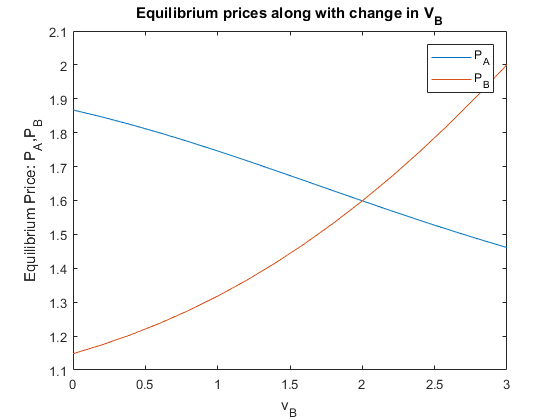
\includegraphics[width=0.7\textwidth]{Problem5.png} 
\end{center}




%%%%%%%%%%%%%%%%%%%%%%
\section*{Matlab Code}
\lstinputlisting{HW2.m}


\end{document}  



  